\documentclass[fleqn]{article}
\usepackage{tikz}
\usepackage{mathtools}

\usetikzlibrary{shapes,arrows,positioning}
\setlength\parindent{0pt}

\begin{document}
\section{Simplest Example}

Let's define the system in Figure~\ref{fig:1}.
Assuming each arrow represents equal probability.
\begin{figure}[h]\centering
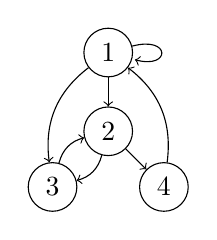
\begin{tikzpicture}
    \node [circle, draw] (p1) {1};
    \node [circle, draw] (p2) [below of=p1] {2};
    \node [circle, draw] (p3) [below left of=p2] {3};
    \node [circle, draw] (p4) [below right of=p2] {4};

    \path[->] (p1) edge [loop right] (p1);
    \path[->] (p1) edge (p2);
    \path[->] (p1) edge [bend right] (p3);

    \path[->] (p2) edge [bend left](p3);
    \path[->] (p2) edge (p4);

    \path[->] (p3) edge [bend left] (p2);

    \path[->] (p4) edge [bend right] (p1);
\end{tikzpicture}\caption{Simplest system.}\label{fig:1}
\end{figure}

A \emph{Markov chain} is a sequence of random variables $X_0,X_1,X_2,...$ taking variables from \emph{state space ${1,2,3,4}$}.

The \emph{transition probability} $q_{ij}$ specifies the probability of going from state $i$ to $j$.

\begin{equation}
q_{ij} = P( X_{n+1}=j | X_n=i )
\end{equation}

The \emph{transition matrix} of the chain is $Q=(q_{ij})$.
\begin{equation}
Q  = \begin{bmatrix}
    1/3 & 1/3 & 1/3 & 0   \\
    0   & 0   & 1/2 & 1/2 \\
    0   & 1   & 0   & 0   \\
    1/2 & 0   & 0   & 1/2 \\
\end{bmatrix}
\end{equation}

Let $q_{ij}^n$ be the \emph{$n$-step transition probability}. It describes the probability of being $j$ after exactly $n$ steps after being at $i$.
\begin{equation}
    q_{ij}^n = P( X_n=j | X_0=i )
\end{equation}

The number can be computed by $Q^n$.

For example,  $q_{13}^5 = 52/243 = 0.2139917695473251$ represents the probability of the chain is in state 3 after 5 steps starting from state.

\end{document}
